%\documentclass[10pt]{article}
\documentclass{sig-alternate}
\pagenumbering{arabic}
\pagestyle{plain}
%\pagestyle{empty}
%\usepackage{fullpage}
%\usepackage{setspace}
%\usepackage[top=2cm,bottom=2cm,left=2cm,right=2cm]{geometry}
%\usepackage{wrapfig}
\usepackage{graphicx}
\usepackage{sidecap}
\usepackage{subfig}
\usepackage{eso-pic,type1cm,color}

% macros to use in the text
\newcommand{\TITLE}{PLFS Roadmap}
\newcommand{\mds}{metadata distribution layer}
\newcommand{\fuse}{PLFS-FUSE}
\newcommand{\adio}{PLFS-ADIO}
\newcommand{\store}{back-end store}
\newcommand{\plfsrc}{\Path{/etc/plfsrc}}

%\newcommand{\summary}[1]{\framebox[6in]{#1}}

\newcommand{\compatibility}[1]{\subsection{Compatibility}{#1}}
\newcommand{\version}[2]{\subsection{Version #1 Summary}{#2}}

\newcommand{\policy}[1]{\summary{Policy Decision}{#1}}
\newcommand{\policyq}[1]{\summary{Policy Question}{#1}}
\newcommand{\implementation}[1]{\summary{Implementation Decision}{#1}}
\newcommand{\implementationq}[1]{\summary{Implementation Question}{#1}}

\newcommand{\summary}[2]{
	\begin{center}
    \begin{tabular}[h!]{|p{0.8\textwidth}|}
    \hline
    {\bf #1}\\\hline
    #2    \\\hline
    \end{tabular}
\end{center}}

\def\sourcetabsize{2}
\newenvironment{sourcestyle}{\begin{scriptsize}}{\end{scriptsize}}
\def\sourceinput#1{\par\begin{sourcestyle}\verbatimtabinput[\sourcetabsize]{#1}\end{sourcestyle}\par}

\newcommand{\Title}[1]{{\bf #1}}
\newcommand{\Term}[1]{{\em #1}}
\newcommand{\eg}{\textit{e.g.}}
\newcommand{\etc}{\textit{etc.}}
\newcommand{\ie}{\textit{i.e.}}
\newcommand{\etal}{\textit{et al.}}
\newcommand{\Math}[1]{$#1$}
\newcommand{\Path}[1]{\textit{#1}}
\newcommand{\RAID}{RAID}
\newcommand{\url}[1]{\textit{#1}}
\newcommand{\syscall}[1]{\textit{#1}}
\newcommand{\plfs}{PLFS}
\newcommand{\noopfs}{No-opFS}
\newcommand{\upfs}{underlying parallel file system}
\newcommand{\rrz}{Roadrunner test cluster}

\newcommand{\KB}{~KB}
\newcommand{\KBs}{~KB/s}
\newcommand{\Kbs}{~Kbit/s}
\newcommand{\mbs}{~Mbit/s}
\newcommand{\MB}{~MB}
\newcommand{\GB}{~GB}
\newcommand{\MBs}{~MB/s}
\newcommand{\GBs}{~GB/s}
\newcommand{\mus}{\mbox{$\mu s$}}
\newcommand{\ms}{\mbox{$ms$}}

\newcommand{\xaxis}{x-axis}
\newcommand{\yaxis}{y-axis}
\newcommand{\mydefinition}[2]{\item {\bf{#1:}} #2}
\newcommand{\figheight}{1.25in}

\newlength{\captwidth} \setlength{\captwidth}{0.9\textwidth}
\newlength{\captsize}  \let\captsize=\footnotesize

\newcommand{\motivationgraph}[2]{
        \subfloat[#1]{\label{fig:#2-motivation}
           \includegraphics[width=0.25\textwidth]{data/#2/#2-motivation.eps}}
}

\newcommand{\readgraph}[3]{
        \subfloat[#1]{\label{fig:#2-read}
           \includegraphics[width=0.25\textwidth]{#3}}
}

\newcommand{\tablefigure}[2]{
    \subfloat[#1]{\label{eval:#2}\includegraphics[width=0.25\textwidth]
        {data/#2/#2.eps}}
}

% works and makes it smaller but it doesn't put it at the bottom of the page
\newcommand{\myfootnotetext}[1]{
    {\begin{minipage}{\captwidth}
    \let\normalsize=\captsize
    \footnotetext{#1}
    \end{minipage}}
}

%\newcommand{\beforecaption}{\vspace{-.15cm}\begin{spacing}{0.85}}
%\newcommand{\aftercaption}{\hrulefill\vspace{-0.45cm}\end{spacing}}
% \newcommand{\aftercaption}{\vspace{-.45cm}\end{spacing}}
\newcommand{\beforecaption}{\vspace{.2cm}}
\newcommand{\aftercaption}{\vspace{-.2cm}}
\newcommand{\mycaption}[3]{
            \beforecaption
            \let\normalsize=\captsize
            \caption[#2]{\label{#1}{{\small \bf #2}}
            {{\small \em #3}\aftercaption}}
}

%\newcommand{\scribble}[1]{{{\marginpar{\tiny#1}}}}
\newcommand{\scribble}[1]{}

%\makeatletter
\AddToShipoutPicture{%
\setlength{\@tempdimb}{.5\paperwidth}%
\setlength{\@tempdimc}{.5\paperheight}%
\setlength{\unitlength}{1pt}%
\put(\strip@pt\@tempdimb,\strip@pt\@tempdimc){%
\makebox(200,-730){{\textcolor[gray]{0.5}%
{\fontsize{.3cm}{.3cm}\selectfont{LANL Technical Release LA-UR 09-02117, \today}}}}
}%
}
\makeatother



\begin{document}
\conferenceinfo{SC09} {November 14--20, Portland, Oregon, USA.}
\CopyrightYear{2009}
\crdata{978-1-60558-744-8/09/11}
\boilerplate{(c) 2009 Association for Computing Machinery. ACM acknowledges that
this contribution was authored or co-authored by a contractor or
affiliate of the U.S. Government. As such, the Government retains a
nonexclusive, royalty-free right to publish or reproduce this article,
or to allow others to do so, for Government purposes only.}
%\doublespace
\title{\TITLE}
\numberofauthors{4}
% Three authors sharing the same affiliation.
    \author{
      \alignauthor John Bent\\      
      \email{johnbent@lanl.gov}
%
     \alignauthor Ben McClelland\\     
      \email{ben@lanl.gov}
%
      \alignauthor James Nunez\\    
      \email{jnunez@lanl.gov}
%
      \alignauthor Meghan Wingate\\    
      \email{meghan@lanl.gov}
%
      \sharedaffiliation
      \affaddr{High Performance Computing }  \\
      \affaddr{Los Alamos National Laboratory } 
          }
%
\date{}
\maketitle
\thispagestyle{empty}
\pagestyle{empty}

\vspace{-.5cm}
\abstract{
\scribble{Rewordings. Eliminated last paragraph. Changed definition of \\upfs to use 'file system' instead of 'file system'. Changed National Science Foundation site to PSC}
\em{
Parallel applications running across thousands of processors must protect
themselves from inevitable component failures. Many applications 
insulate themselves from failures by checkpointing, a
process in which they save their state to persistent storage. Following a
failure, they can resume computation using this state.
For many applications, saving this state into a shared single file
is most convenient.  With such an approach, the size of writes are often 
small and not aligned with file system boundaries. Unfortunately for these
applications, this preferred data layout results in pathologically poor
performance from the underlying file system which is optimized for
large, aligned writes to non-shared files.
\if 0
% Milo's changes which I didn't incorporate
process in which they periodically save their state to persistent storage. Following a
failure, they can retrieve the most recently saved state and resume computation from that
point. For many applications, saving this state into a shared single file, often
formatted for storage by complex libraries such as NetCDF or HDF5,
is most convenient.  With such an approach, the size of individual write system calls are often 
small and not aligned with file system boundaries especially when the application cannot statically define the order of state variables, as with adaptive mesh refinement app. Unfortunately for these
applications, this write access pattern can result in pathologically poor
performance from an underlying file system, itself often optimized for
\fi
 
To address this fundamental mismatch, we have developed a parallel
log-structured file system, \plfs, which is positioned between the applications
and the \upfs. \plfs\ remaps an application's write access pattern to be
optimized for the underlying file system. Through testing on Panasas
ActiveScale Storage System and IBM's General Parallel File System at Los Alamos
National Lab and on Lustre at Pittsburgh Supercomputer Center, we have seen
that this layer of indirection and reorganization can reduce checkpoint time by
up to several orders of magnitude for several important benchmarks and real
applications. 
 
We expect that \plfs\ can improve the checkpoint bandwidth for any large
parallel application that writes to a single file. The expected improvement is
especially large for those applications doing unaligned or random IO, patterns
which have become increasingly prevalent recently due to the wide-spread
adoption of complex formatting libraries such as NetCDF and HDF5. 

\if 0
% here's the 150 word limited version we submitted to SC
Parallel applications running across thousands of processors must protect themselves from inevitable system failures. Many applications insulate themselves from failures by checkpointing. For many applications, checkpointing into a shared single file is most convenient. With such an approach, the size of writes are often small and not aligned with file system boundaries. Unfortunately for these applications, this preferred data layout results in pathologically poor performance from the underlying file system which is optimized for large, aligned writes to non-shared files. To address this fundamental mismatch, we have developed a virtual parallel log structured file system, PLFS. PLFS remaps an application’s preferred data layout into one which is optimized for the underlying file system. Through testing on PanFS, Lustre, and GPFS, we have seen that this layer of indirection and reorganization can reduce checkpoint time by an order of magnitude for several important benchmarks and real applications.
\fi
}
}

\category{D.4.3}{Operating Systems}{File Systems Management}{File organization}
\terms{Performance, Design}
\keywords{High performance computing, parallel computing, checkpointing}
\section{Introduction}

\scribble{Need to define "its class" --Milo}
% computers are large, they have failures
In June 2008, Los Alamos National Labs (LANL), in partnership with IBM, broke
the petaflop barrier and claimed the top spot on the Top 500 list~\cite{top500}
with the Roadrunner supercomputer~\cite{roadrunner}.  Due to its unique hybrid
architecture, Roadrunner has only 3060 nodes, which is a relatively small
number for a supercomputer of its class.  Unfortunately, even at this size,
component failures are a frequent event.  These failures are particularly
problematic as many applications at LANL, and other High Performance Computing
(HPC) sites, have long run times in excess of days, weeks, and even months.

% checkpoint is defense against failure, drives parallel file systems, is
% challengin
Typically these applications protect themselves against failure by periodically
\Term{checkpointing} their progress by saving the state of the application to
persistent storage. After a failure the application can then restart from the most recent 
checkpoint.  Due to the difficulty of reconstructing a consistent
image from multiple asynchronous checkpoints~\cite{lamport1978}, HPC
applications checkpoint synchronously (\ie\ following a barrier).  Synchronous
checkpointing, however, does not eliminate the complexity; it merely shifts it to
the parallel file system which now must coordinate simultaneous access from
thousands of compute nodes.  Even using optimal checkpoint frequencies~\cite{daly-optimal}, 
checkpointing has become the driving workload for
parallel file systems and the challenge it imposes grows with each successively
larger supercomputer~\cite{pcl:99:me,schroeder2007}.  The difficulty of this
challenge can vary greatly depending on the particular pattern of checkpointing
chosen by the application. 

% our approach
In this paper, we describe different checkpointing patterns, and show how some
result in very poor storage performance on three of the major HPC
parallel file systems: PanFS, GPFS, and Lustre.  We then posit that an
interposition layer inserted into the existing storage stack can rearrange this
problematic access pattern to achieve much better performance from the
\upfs.  To test this hypothesis, we have developed \plfs, a Parallel
Log-structured File System, which is one such interposition layer.  We present measurements using \plfs\ on several synthetic benchmarks and real applications at multiple HPC supercomputing centers.  The
results confirm our hypothesis: writing to the \upfs\ through
\plfs\ improves checkpoint bandwidth for all tested applications and
benchmarks and on all three studied parallel file systems; in some cases,
bandwidth is raised by several orders of magnitude.

\begin{figure}
    \centering
    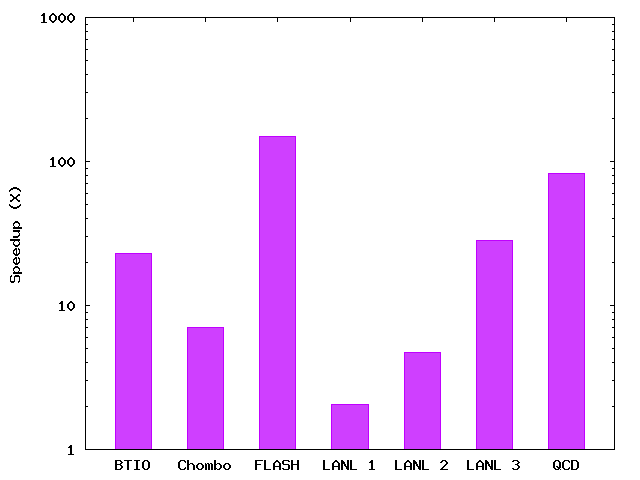
\includegraphics[width=0.4\textwidth]{data/summary/page1.eps}
    \mycaption{fig-page1}{Summary of our results.}{
        This graph summarizes our results which will be
        explained in detail in Section~\ref{eval}.  
        The key observation here is that our technique
        has improved checkpoint bandwidths for all seven
        studied benchmarks and applications by up to
        several orders of magnitude.  
        \vspace{1.0cm}
    }
\end{figure}


As we shall discuss, and is summarized in Figure~\ref{fig-page1}, PLFS is
already showing very large speed ups for widely used HPC benchmarks and
important real HPC codes, and at extreme scale. 

% the stupid mandatory list of the rest of the paper
The rest of the paper is organized as follows.  We present more detailed background and
motivation in Section~\ref{motivation}, describe our design in
Section~\ref{arch} and our evaluation in Section~\ref{eval}.  We present
related work in Section~\ref{related}, current status and future work in
Section~\ref{future}, and finally we conclude in Section~\ref{conclude}.

\section{Background}
\label{motivation}

% Why do we care about checkpointing
\if 0
As a result, applications 
periodically save
the current state of their computation to persistent storage.  Later, after a
failure is encountered, the application can restart from the last saved
checkpoint. 
\fi

% N-N compared to N-1

\scribble{Lots of tweaking of final sentence} 
From a file system perspective,
there are two basic checkpointing patterns: ~\Term{N-N} and ~\Term{N-1}.  An
N-N checkpoint is one in which each of ~\Math{N} processes writes to a unique
file, for a total of ~\Math{N} files written.  An N-1 checkpoint differs in
that all of ~\Math{N} processes write to a single shared file.  Applications
using N-N checkpoints usually write sequentially to each file, an access
pattern ideally suited to parallel file systems. Conversely, applications using
N-1 checkpoint files typically organize the collected state of all N processes
in some application specific, canonical order, often resulting in 
small, unaligned, interspersed writes.

Some N-1 checkpoint files are logically the equivalent of concatenating the
files of an N-N checkpoint (\ie\ each process has its own unique region
within the shared file).  This is referred to as an ~\Term{N-1 segmented}
checkpoint file and is extremely rare in practice.  More common is an
~\Term{N-1 strided} checkpoint file in which the processes write multiple small
regions at many different offsets within the file; these offsets are typically
not aligned with file system block boundaries~\cite{plfs-maps}.  N-1 strided
checkpointing applications often make roughly synchronous progress such that
all the processes tend to write to the same region within the file concurrently, and collectively this region sweeps across the file.
These three patterns, N-N, N-1 segmented, and N-1 strided, are
illustrated in Figure~\ref{fig-patterns}.  Since N-1 segmented is a rare pattern
in practice, hereafter we consider only N-1 strided and we refer to it with the
shorthand N-1. 

\scribble{Should probably explain or remove 'false sharing' in figure}
\scribble{If those Argonne graphs were decipherable in B-W, I'd like to include
two of them to visualize the difference between strided and non.}

% file system challenges for N-N and N-1
The file system challenge for an N-N workload is the concurrent creation of
thousands of files which are typically within a single directory.  An N-1
workload can be even more challenging however for several different reasons
which may depend on the particular parallel file system or the underlying
\RAID\ protection scheme.  In the Panasas ActiveScale parallel
file system~\cite{Welch04managingscalability} (PanFS), for example, small strided
writes within a parity stripe must serialize in order to maintain consistent
parity.  In the Lustre parallel file system~\cite{lustre}, writes to N-1
checkpoint files which are not aligned on file system block boundaries cause
serious performance slowdowns as well~\cite{nersc}.  Although both
N-N and N-1 patterns pose challenges, it has been our observation, as well
as that of many others~\cite{grider-hec,adios,nersc,zest,Thakur99datasieving},
that the challenges of N-1 checkpointing are more difficult. 
Applications using N-1 patterns consistently achieve significantly less
bandwidth than do those using an N-N pattern. 

\begin{figure*}[tb]
    \centering
        \motivationgraph{PanFS}{panfs}
        \motivationgraph{GPFS}{gpfs}
        \motivationgraph{Lustre}{lustre}
    \\
    \mycaption{fig-motivation}{Motivation.}{
These three graphs demonstrate the large discrepancy between achievable
bandwidth and scalability using N-N and N-1 checkpoint patterns on three of 
the major HPC parallel file systems. 
    }
\end{figure*}



Figure~\ref{fig-motivation} presents experimental data validating this
discrepancy: An N-1 checkpoint pattern receives only a small fraction of the
bandwidth achieved by an N-N pattern on PanFS, GPFS, and Lustre and does not
scale with increased numbers of nodes.  The PanFS experiment, run on LANL's
Roadrunner supercomputer using its 1000 blade PanFS storage system, shows a
maximum observed N-N bandwidth of 31~\GBs\ compared to a maximum observed N-1
bandwidth of less than 100~\MBs.  Although we show PanFS results using their
default RAID-5 configuration, PanFS has also a RAID-10 configuration which
reduces the implicit sharing caused by N-1 patterns when two writers both need
to update the same parity.  While this solution improves scaling and offers
much higher N-1 write bandwidth without sacrificing reliability, it does so by
writing every byte twice, a scheme that, at best, can achieve only
approximately half of the write bandwidth of N-N on RAID-5.  \plfs, however, as
will be shown in Section~\ref{eval}, can get much closer.

The GPFS and Lustre experiments were run on much smaller systems. The GPFS
experiment was run using an archive attached to Roadrunner using its 
nine, quad-core, file transfer nodes.  The Lustre experiment was run using five
client machines, each with eight cores, and twelve Lustre servers.  All three
file systems exhibit similar behavior; N-N bandwidths are consistently higher
than N-1 by at least an order of magnitude.  Measurements were gathered using
the LANL synthetic checkpoint tool, \Term{MPI-IO Test}~\cite{mpi-io-test}.
For each of these graphs, the size of each \syscall{write} was
47001 bytes (a small, unaligned number observed in actual applications to be
particularly problematic for file systems). \syscall{Writes} were
issued until two minutes had elapsed. Although this is atypical since 
applications tend to write a fixed amount of data instead of writing for
a fixed amount of time, we have observed that this allows representative 
bandwidth measurements with a predictable runtime. 

% why all applications not N-N
Since N-N checkpointing derives higher bandwidth than N-1, the obvious path to
faster checkpointing is for application developers to rewrite existing N-1
checkpointing applications to do N-N checkpointing instead.  Additionally, all
new applications should be written to take advantage of the higher bandwidth
available to N-N checkpointing.  Although some developers have gone this route,
many continue to prefer an N-1 pattern even though its disadvantages are well
understood.  There are several advantages to N-1 checkpointing that appeal to
parallel application developers.  One, a single file is much easier to manage
and to archive.  Two, N-1 files usually organize data into an application
specific canonical order that commonly aggregates related data together in
contiguous regions, making visualization of intermediate state simple and
efficient.  Additionally, following a failure, a restart on a different number
of compute nodes is easier to code as the checkpoint format is independent of
the number of processes that captured the checkpoint; conversely, gathering the
appropriate regions from multiple files or from multiple regions within a
single file is more complicated.  

% a list of some apps that do N-1

Essentially these developers have once again shifted complexity to the parallel
file system for their own convenience.  This is not unreasonable; it has long
been the province of computer systems to make computing more convenient for its
users.  Many important applications have made this choice.  Of the twenty-three
applications listed on the Parallel I/O Benchmarks page~\cite{pio-benchmarks},
at least ten have an N-1 pattern; two major applications at LANL use an N-1
checkpointing pattern as do at least two of the eight applications chosen to
run on Roadrunner during its initial stabilization phase.  N-1 checkpointing is
very important to these applications.  For example, at the core of one of
LANL's N-1 applications is a twenty-year old Fortran checkpointing library. 
About a decade ago, in response to a growing clamor about the
limitations of N-1 checkpointing bandwidth, developers for this application
augmented their checkpointing library with fifteen thousand lines of code.
However, instead of changing the application to write an N-N pattern, they
added a prefer to the IO routiones in which interprocess communication is used to aggregate and buffer writes.
Although they did not improve the performance to match that of other 
applications using an N-N checkpoint pattern, 
this effort was considered a success as they did improve the N-1
performance by a factor of two to three. This new checkpointing library,
called \Term{bulkio}, has been maintained over the past decade and ported to
each new successive supercomputer at LANL~\cite{bent-personal-bulk}. 
Furthermore, N-1 patterns continue to be developed anew in many new
applications.  High level data formatting libraries such as Parallel
NetCDF~\cite{pnetcdf} and HDF5~\cite{hdf5} offer convenience to application
developers who simply describes the logical format of their data and need no
longer consider how that data is physically organized in the file system.  Once
again this convenience merely shifts the complexity to the \upfs\ 
since these libraries use an N-1 pattern.


% Milo's change which I didn't like
%More generally, parallel application developers employ data formatting libraries such as NetCDF~\cite{pnetcdf} and HDF5~\cite{hdf5} to simplify programming, but these extra layers of mapping can lead to decreased locality and sequentiality when checkpointing a logically related set of variables. N-1 write access patterns can appear in new applications this way.

\section{Design of an Interposition Layer}
\label{arch}

\begin{figure*}[tb]
    \centering
    \subfloat[\label{typical}Typical Experiment Lifecycle]{
        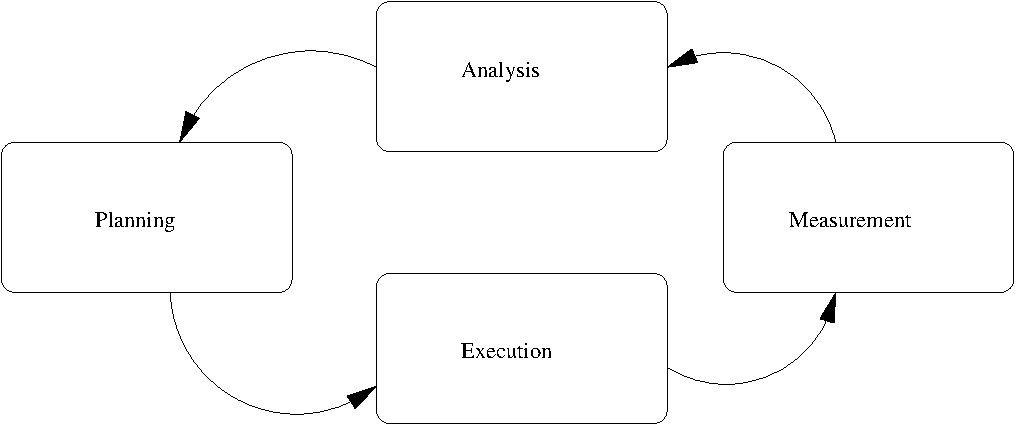
\includegraphics[width=0.4\textwidth]{figs/planning.pdf}
    }
    \hspace{0.5in}
    \subfloat[\label{lem-plan}\name\ Augmented Experiment Lifecycle]{
        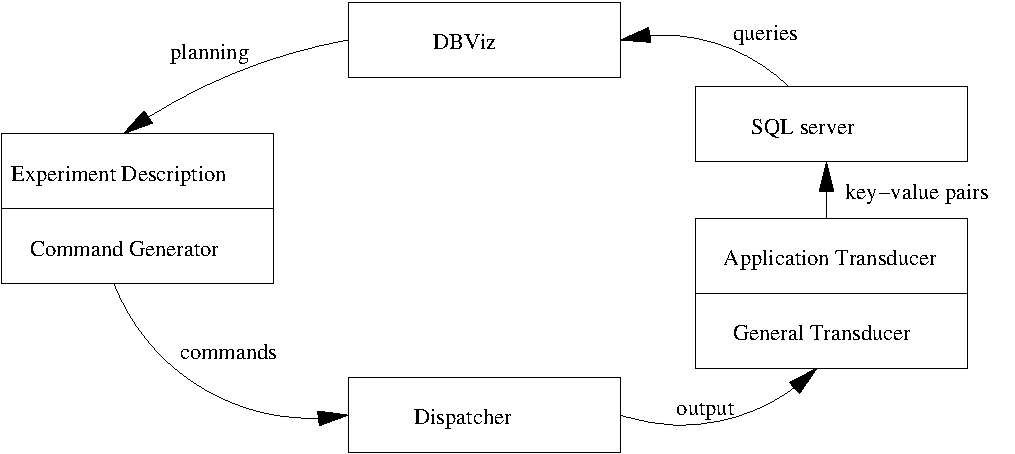
\includegraphics[width=0.4\textwidth]{figs/arch.pdf}
    }
    \mycaption{fig-plan}{Experiment Lifecycle.}{
The figure on the left depicts a typical experiment lifecycle progressing
through planning, execution, measurement, and analysis.  A user devises an
experiment to study the effect of some number of independent variables,
executes and measures each \sub, analyzes the results, and, depending on that
analysis, can then revise the experiment and repeat the cycle.  The figure on
the right shows the workflow within \name.  The user describes their parameter
space to the \cg\ and specifies a path to an optional application transducer to
capture application specific \kv\ pairs.  \name\ adds a path to a general
transducer to capture \kv\ pairs common to all experiments.  The generated
commands and their transducer(s) are then passed to the \dispatcher\ which
either submits the commands to a scheduling system or runs them synchronously
in the foreground.  As the commands run, \kv\ pairs are captured by the
transducer(s) and inserted into a SQL server from which they can then be
queried to visualize and analyze the results.  Depending on this analysis the
user can then modify their parameter space and repeat the cycle.
}
\end{figure*}


We start with the hypothesis that an interposition layer can transparently
rearrange an N-1 checkpoint pattern into an N-N pattern and thereby decrease
checkpoint time by taking advantage of the increased bandwidth achievable via
an N-N pattern. To test this hypothesis, we have developed one such
interposition layer, \plfs, designed specifically for large parallel N-1
checkpoint files. The basic architecture is illustrated in
Figure~\ref{fig-arch}. \plfs\ was prototyped with FUSE~\cite{fuse}, a 
framework for running stackable file systems~\cite{usenix00fist} in 
non-privileged mode.


\plfs\ is a virtual FUSE file system, mounted on the compute nodes, situated between the parallel application and
an \upfs\ responsible for the actual data storage. 
As \plfs\ is a virtual file
system, it leverages many of the services provided by the \upfs\ such as
redundancy, high availability, and a globally distributed data store.  This
frees \plfs\ to focus on just one specialized task: rearranging application
data so the N-1 write pattern is better suited for the \upfs.  In the remainder
of this paper,  we refer to \plfs\ generally to mean this virtual file system
which itself is comprised of a set of \plfs\ servers running across a compute
system bound together by an \upfs; when we refer to a {\em specific} \plfs\ we
mean just one of these servers.

\scribble{Cut last sentence --Milo}

% Although \plfs\ looks and feels like a
%full-fledged parallel file system, in actuality it is merely a collection of
%independent virtual file systems running on each compute node that appear
%parallel only because they exploit the parallelism of the underlying
%file system.

%As multiple processes in a parallel application open an N-1 checkpoint file,

\subsection{Basic operation}
The basic operation of \plfs\ is as follows. For every logical \plfs\ file
created, \plfs\ creates a \Term{container} structure on the \upfs. Internally,
the basic structure of a container is a hierarchical directory tree consisting
of a single top-level directory and multiple sub-directories that appears to
users; \plfs\ builds a logical view of a single file from this container
structure in a manner similar to the core idea of Apple
bundles~\cite{bundles} in Mac OS X.  Multiple processes opening the same
logical file for writing share the container although each open gets a unique
\Term{data file} within the container into which all of its writes are
appended. By giving each writing process in a parallel application access to a
non-shared data file, \plfs\ converts an N-1 write access pattern into a N-N
write access pattern.  When the process writes to the file, the write is
appended to its data file and a record identifying the write is appended to an
index file (described below). 

\scribble{Added words, Mac OS X citation}

\subsubsection{Reading from \plfs}
\label{arch-read}
Rearranging data in this manner should improve write bandwidths, but
it also introduces additional complexity for reads. In order to read 
the logical file, \plfs\ maintains an \Term{index file} for each compute
node which records the logical offset and length of each write. \plfs\ can
then construct a \Term{global index} by aggregating the multiple index files 
into an offset lookup table.  This global offset is constructed as needed to
satisfy read operations and lookup operations when cached metadata is not
available (as will be discussed in Section~\ref{arch-meta}).

One difficultly in constructing this global index stems from concurrent
processes that may write the same offset at the same time.  These processes
cannot know which will be the ultimate writer, so they need to synchronize to
determine the appropriate order. This synchronization needs to be exposed to
the file system to be effective~\cite{Gibson95thescotch}. If a logical
clock~\cite{lamport1978} was associated with these synchronizations, its value
could be written to index files so that the merge process could correctly
determine write ordering. Since parallel applications synchronize with a
barrier called by all processes, a simple count of synchronization calls could
be sufficient. In practice checkpoints do not experience overlapping writes, so
at this time \plfs\ has not implemented an overlap conflict resolution scheme.

\scribble{changed language on 'serialization of index writes'. We actually only
serialize the index offset updates --Milo} 

One interesting nuance is that \plfs\ has a data file for every process but
only a single index file per compute node shared by all processes on that node.
Sharing an index file is easy; by the time \plfs\ sees writes, they have been
merged by the operating system into a single memory space. The operating
systems sends all writes to a single \plfs\ process which ensures index records
are correctly, chronologically appended.  Having a single index greatly reduces
the number of files in a container since current LANL applications run up to
sixteen processes on a node; on the next LANL supercomputer, this could be up
to sixty-four. We tried reducing the number of data files in the same manner.
Write bandwidth was not affected, but reads were slowed for \Term{uniform
restarts} in which reading processes access the file in the same access pattern
as it was written.  The pattern of a single reader accessing a single data file
sequentially lends itself very well to prefetching.  However, due to timing
differences between the write and read phases, multiple processes in a uniform
restart may not always read from a shared file in sequential order.

Having described the basic operation of \plfs, we now present some of its
implementation in finer detail.  Although there are many interposition
techniques available (~\cite{bypass} includes a survey), we have selected FUSE
for several reasons. Because FUSE allows \plfs\ to be accessible via a standard
file system interface, applications can use it without modification and files on
\plfs\ can be accessed by the entire suite of existing tools such as
\textit{ls}, \textit{diff}, and \textit{cp}. In addition to providing user
transparency, using FUSE dramatically simplified our development effort. A file
system in userspace is significantly easier to develop than a kernel file
system and is more portable as well. However, this convenience is not free as
FUSE does add some overhead as shown in Section~\ref{eval}. 

\subsubsection{Container implementation}

\scribble{I think this part was superfluous so I cut the LD\_PRELOAD stuff}
%Finally, the simplified interface
%of the FUSE API means developers need only implement a small subset of
%function calls as opposed to the much larger set that would be required if
%we had chosen to interpose using an \textit{LD\_PRELOAD} library. As will
%be shown however in Section~\ref{eval}, this convenience is not free as FUSE
%does add some small amount of overhead. 

Because \plfs\ leverages the \upfs\ as much as possible, we give the container
the same logical name as the \plfs\ file. This allows \plfs\ to pass a
\syscall{readdir} system call directly to the \upfs\ and return its result to
the application without any translation.  \plfs\ also handles \syscall{mkdir}
system calls in the same way (\ie\ without any translation). The implication of
leveraging the \upfs\ in this way is that \plfs\ requires some other mechanism
by which to distinguish between regular directories and containers in order to
implement the \syscall{stat} system call correctly. As the \textit{SUID} bit is
rarely used on directories and yet is allowed to be set by the underlying file
system, \plfs\ sets this bit on containers; this does mean, however, that
\plfs\ must disallow setting this bit on a regular directory. 

As we discussed previously, parallel applications do synchronized
checkpointing; the implication for \plfs\ is that multiple processes running on
multiple compute nodes writing an N-1 checkpoint file will cause
\plfs\ on each compute node to attempt to create the same container
concurrently on the \upfs. The difficulty arises because each \plfs\ must first
\syscall{stat} that path to see whether the path is available, whether that
container already exists, or whether there is a regular directory at that
location. Ideally, each \plfs\ could \syscall{stat} the path and, when the
location is empty, atomically create a
directory with the \textit{SUID} bit set. Unfortunately, the \syscall{mkdir}
system call ignores the \textit{SUID} bit; each \plfs\ must therefore first
create a directory and then set the \textit{SUID} bit. Doing this
naively results in a race condition: if one \plfs\ \syscall{stats} the path
after another has made the directory but before it has set the \textit{SUID}
bit, then the \syscall{stat} will indicate that there is a regular directory in
that location. The application issuing the open of the logical file will then
receive an error incorrectly indicating that there is a directory already at
that location. To avoid this race condition, each \plfs\ first makes a
hidden directory with a unique name, set its \textit{SUID} bit, and then
atomically \syscall{renames} it to the original container name.

\subsection{Metadata operations}
\label{arch-meta}

Metadata operations against a file include accessing its permissions (including
SUID), its capacity, the offset of its last byte and the timestamp of its last
update. For a directory on \plfs, these are provided by the underlying
file system. But for a \plfs\ file which is constructed from a container like
the example in Figure~\ref{fig-arch}, these metadata operations have to be
computed from the many underlying files within the container.

Because the SUID bit on the container itself has been overloaded to indicate
that the directory is not a directory at all, but rather a container, it cannot
be also used to indicate if the user has set SUID on the \plfs\ file
represented by the container. Instead we use a file inside the container, the
\Term{access file}, to represent the appropriate SUID and the rest of the
permissions associated with the container. For example, where \syscall{chmod}
and \syscall{chgrp} are directed at the logical file, they are applied to the
access file within the container.

Capacity for the logical file is the sum of the capacities of the files inside
the container.  The last update timestamp is the maximum of the last update
timestamps.  And the offset of the last byte is the maximum logical offset
recorded in any of the index files.

Computing these sums and maximums with every \syscall{stat} call on a \plfs\
file is expensive. Our strategy for speeding this up is to cache recently
computed values in the \Term{metadata subdirectory}. To make this cache as
effective as possible we have each FUSE process cache into this metadata
subdirectory any information it has in its in memory data structures when the
last writer on that node closes the file. On this close, the
FUSE process creates a file named H.L.B.T, where H is the node's hostname, L is
the last offset recorded on that node, B is the sum of the capacity of all
files that this node manages, and T is the maximum timestamp among these files.

When no process has this container open for write, a stat call on the container
is implemented by issuing a \syscall{readdir} on the metadata subdirectory,
then reporting the maximum of the Ls for last byte offset, the maximum of the
Ts for modification timestamp and the sum of the Bs for capacity.

If one or more processes has the container open for writing, then the
corresponding cached metadata values could be stale. \plfs\ clients therefore
create a file in the \Term{openhosts subdirectory} named by its hostname when
one or more processes on that node have that file open for writing, and
then deleting this file once all \syscall{opens} have been closed.
\syscall{stat} must then do a \syscall{readdir} on openhosts as well to
discover if any node has the file open for writing, and thereby determine which
metadata cache entries might be stale.

When there are hostname files in the openhosts subdirectory, the node that is
executing the \syscall{stat} call could read the contents of the index files
associated with those hostnames in order to find the largest logical offset,
and then combine this with the metadata cache files that are not stale.

In the experience of the HPC community, \syscall{stat'ing} an open file is
almost always done by a user trying to monitor the progress of their job. What
they want is an inexpensive probe showing progress, not an expensive
instantaneously correct value~\cite{hec-posix}. Following this logic, \plfs\
does not read and proccess the index files associated with hostnames that have
the container open for write. Instead it assumes that files are not sparse
(\ie\ every byte has been written) and sums the sizes of all data files within
a container to estimate the last offset of the \plfs\ file.  Because writes to
each data are always simply appended, this estimation will monotonically
increase as additional data is written into the file, allowing users to monitor
progress. When the container is closed, the metadata subdirectory contains
fully correct cached values, and full accuracy is provided at all times when
the container has no processes writing it.

\section{Evaluation}
\label{eval}

% eval figures all in one big table
\begin{figure*}[t!]
\centering
\begin{tabular}{ccc}
    \tablefigure{MPI-IO Test on PanFS}{panfs}
    &
    \tablefigure{MPI-IO Test on GPFS}{gpfs}
    &
    \tablefigure{MPI-IO Test on Lustre}{lustre}
    \\
    \tablefigure{LANL Anonymous 1}{lanl1}
    &
    \tablefigure{LANL Anonymous 2}{lanl2}
    &
    \tablefigure{LANL Anonymous 3}{lanl3}
    \\
    \tablefigure{PatternIO}{pattern}
    &
    \tablefigure{QCD}{qcd}
    &
    \tablefigure{BTIO}{btio}
    \\
    \tablefigure{FLASH IO}{flash}
    &
    \tablefigure{SUMMARY}{summary}
    &
    \tablefigure{Chombo IO}{chombo}
\end{tabular}
\mycaption{fig-eval}{Experimental Results.}{
The three graphs in the top row are the same graphs that were presented
earlier in Figure~\ref{fig-motivation}, except now they have an additional
line showing how PLFS allows an N-1 checkpoint to achieve most, if not all,
of the bandwidth available to an N-N checkpoint. 
The bar graph in the center of the bottom row consolidates these results and
shows a pair of bars for each, showing both the relative minimum and the
maximum speedups achieved across the set of experiments.  Due to radically
different configurations for these various experiments, the axes for 
these graphs are not consistent.  The relative comparison within each graph
should be obvious; absolute values can be ascertained by reading the axes.
}
\end{figure*}


We present the results of our experimental evaluation in Figure~\ref{fig-eval}.
Eleven of these twelve graphs present one experiment each. The twelfth,
Figure~\ref{eval:summary}, presents a summary. In the majority of these graphs,
the write bandwidth is shown on the \yaxis\ in \MBs\ as a function of the
number of processes. We will note it in the text for those few graphs for
which we deviate from this general configuration. The write bandwidth that we
report is whatever is reported by the particular benchmark; whenever possible,
we report the most conservative value (\ie\ we include open and close times in
our write times, and we either barrier after close or we use the time reported
by the slowest writer). Finally we have attempted to run multiple iterations
for each experiment; where applicable, the standard deviation is therefore
included.

\subsection{MPI-IO Test}

The top three graphs, 
Figures~\ref{eval:panfs},~\ref{eval:gpfs},~and~\ref{eval:lustre}, present the
results of our study using the LANL synthetic checkpoint tool, \Term{MPI-IO
Test}~\cite{mpi-io-test}, on three different parallel file systems, PanFS, GPFS,
and Lustre. For each of these graphs, the size of each \syscall{write} was
47001 bytes (a small, unaligned number observed in actual applications to be
particularly problematic for file systems). \syscall{Writes} were
issued until two minutes had elapsed. Although this is atypical since 
applications tend to write a fixed amount of data instead of writing for
a fixed amount of time, we have observed that this allows representative 
bandwidth measurements with a predictable runtime. 

There are several things to notice in these graphs. The first is that these
are the same three graphs that we presented in Figure~\ref{fig-motivation}
except that we have now added a third line to each. The three lines show the
bandwidth achieved by writing an N-N pattern directly to the \upfs, the
bandwidth achieved by writing an N-1 pattern directly to the \upfs, and the
third line is the bandwidth achieved by writing an N-1 pattern {\em indirectly}
to the \upfs\ through \plfs.

These graphs illustrate how the performance discrepancy between N-N
and N-1 checkpoint patterns is common across PanFS, GPFS,
and Lustre. Remember, as was discussed in Section~\ref{motivation}, switching
to N-N is not a viable option for many applications which are inextricably wed
to an N-1 pattern and are resigned to the attendant loss of bandwidth.
Fortunately, as is evidenced by these graphs, \plfs\ allows these applications
to retain their preferred N-1 pattern while achieving most, if not all, of the
bandwidth available to an N-N pattern. Particularly for the PanFS results,
which were run on our Roadrunner supercomputer, \plfs\ achieves the full
bandwidth of an N-N pattern (\ie\ up to about 31 \GBs). In fact, for several
of the points, an N-1 pattern on \plfs\ actually outperforms an N-N pattern
written directly to PanFS. Although we have yet to fully investigate the exact
reason for this, there are several reasons why this could be the case. The
first is that \plfs\ rearranges writes into a log structured pattern so an N-N
pattern which incurs seeks could do worse than a \plfs\ pattern which appends
only. Secondly, the structure of the \plfs\ container spreads data across
multiple sub-directories within a top-level directory whereas a typical N-N
pattern confines all N files into only a single parent directory.

Although \plfs\ does improve the bandwidth of N-1 patterns on GPFS and Lustre,
the improvement is not as large as it is on PanFS. This is because the scale
of the experiments on PanFS are 200 times larger than on the other two
platforms. In the inset in Figure~\ref{eval:panfs} at the extreme low values
for the number of processes, we see that \plfs\ does not scale N-1 bandwidth
as fast as N-N scales for PanFS as well. This is due to overheads incurred by
both FUSE and \plfs; these overheads limit the total bandwidth achieved by any
single compute node relative to N-N. For HPC systems at extreme scale this
limitation does not matter since aggregate bandwidth across multiple nodes is
more relevant than the bandwidth from a single node. In this case the real
limiting factor is the total bandwidth capacity of the storage fabric, which
generally saturates when using only a small fraction of compute nodes.
However, with poorly-behaved IO patterns (\ie\ N-1), even very large jobs may
not reach these bandwidth limits because they will be more severely
constrained by file system limitations as exemplified by
Figure~\ref{fig-motivation}. \plfs\ is designed to remove these file system
limitations, so that jobs can achieve higher bandwidth and reach the
same limitation of the storage fabric which is constraining N-N bandwidth. 
 
An unusual feture of the inset graph in Figure~\ref{eval:panfs} is that there
are localized bottlenecks about 700 processes.  This is due to the
architecture of Roadrunner and it's connection to PanFS.  Roadrunner is split
into seventeen sub-clusters, \Term{CUs}, each of which can run 720 proceses.
The CUs are fully connected via an Infiniband fat tree, however, in order to
minimize network infrastructure costs, the storage system is partitioned into
multiple sub-nets. Each CU currently has six specialized IO nodes, one for
each sub-net; these six IO nodes are the storage bandwidth bottleneck.
Therefore, as a job grows within a CU, it quickly saturates the IO node
bandwidth; when it grows into another CU, its bandwidth increases sharply due
to gaining six additional IO nodes: this explains the "stair-step" behavior of
the N-N and \plfs\ lines in this graph. 
 
We do see this same behavior in our GPFS and Lustre graphs, but due to the
very small size of our test systems, we do not have enough compute nodes to
saturate the available storage bandwidth and thus neither the N-N nor the
\plfs\ lines in these graphs reach a storage bandwidth bottleneck. We will
examine the FUSE and PLFS overheads in greater detail in
Section~\ref{overhead}. 

\subsection{Real LANL Applications}

The second row in Figure~\ref{fig-eval}, consisting of
Figures~\ref{eval:lanl1},~\ref{eval:lanl2},~and~\ref{eval:lanl3}, shows the
results of using \plfs\ to improve the bandwidth of three important LANL
applications which use N-1 checkpoint patterns. The application
shown in Figure~\ref{eval:lanl1} is the application whose developers augmented
their checkpoint routine with a new checkpoint library called bulkio, which
aggregates and buffers writes into larger, contiguous writes more friendly to
the \upfs. Therefore we show four lines in this graph: one for the old
checkpoint method which uses MPI-IO routines to directly write data to PanFS, a
line for the bulkio method writing directly to PanFS, and a second line for
each of these techniques writing indirectly to PanFS via \plfs. Notice that
\plfs\ is not able to improve the bulkio technique which loses a significant
amount of bandwidth due to aggregating data and reducing parallelism by
reducing the number of writers. However, when the older MPI-IO technique is
used with \plfs, \plfs\ is able to exploit the additional parallelism possible
by using all of the processes as writers. This data was collected on a small,
Opteron-only, \rrz. The next two graphs show similar results; using \plfs\ to
rearrange an N-1 pattern yields significantly improved bandwidths.
Figure~\ref{eval:lanl2} was also run on the \rrz, whereas
Figure~\ref{eval:lanl3} was run on Roadrunner itself; this can be seen by the
much larger scale (on both the \yaxis\ and the \xaxis) for
Figure~\ref{eval:lanl3}. Note that hese are extremely important applications
at LANL; it has been estimated that they account for more than half of the
total computing cycles at LANL. Although these applications must remain
anonymous, traces of their IO are available~\cite{plfs-maps}.

\subsection{NERSC's PatternIO Benchmark}

Figure~\ref{eval:pattern} presents the data derived from our measurements taken
using NERSC's PatternIO benchmark~\cite{nersc} which plots write bandwidth as a
function of \syscall{write} size. Notice that this deviates from the other
graphs in Figure~\ref{fig-eval} which plot write bandwidth as a function of the
number of processes. For this experiment, run on the \rrz, the number of
processes was set at a constant 512. This graph also is a scatter plot instead
of using lines with standard deviations. The points for writing directly to
PanFS show three interesting slopes all converging at about 1 GB/s on the far
right side of the graph. The highest of these three regions shows the
performance of \syscall{writes} when the write size is both block aligned and
aligned on file system boundaries. The middle region is when the write size is
block aligned only and the lowest region is when the write size is not aligned
at all. {\em This graph demonstrates that \plfs\ allows an application to
achieve a consistently high level of write bandwidth regardless of the size, or
alignment, of its \syscall{writes}.}

\subsection{Other Benchmarks}

The remainder of the graphs show various other parallel IO benchmarks with an
N-1 checkpoint pattern. QCD~\cite{qcd-io} in Figure~\ref{eval:qcd} shows a
large improvement using \plfs\ but this improvement actually {\em degrades} as
the number of processes increases. This is because the amount of data written
by QCD is a small constant value and the overhead due to container creation
incurred in the \syscall{open} becomes proportionally greater as the amount of
data written by each process decreases. BTIO~\cite{btio-io} in
Figure~\ref{eval:btio} also shows a large improvement but we currently only
have one data point; we will have more in the final version.
FLASH~IO~\cite{flash-io} and Chombo~IO\cite{chombo-io}, shown respectively in
Figures~\ref{eval:flash}~and~\ref{eval:chombo}, both show improvement due to
\plfs\ which scales nicely with an increasing number of processes. FLASH was
run on Roadrunner whereas Chombo was run on the \rrz; both were built with the
HDF5 library~\cite{hdf5}.

\subsection{Summary}

A summary of the benchmark results, excluding the LANL and NERSC synthetics, is
presented in Figure~\ref{eval:summary}. This summary shows a pair of bars for
each benchmark; one for both the worst-case and best-case speedups for \plfs.
Only in one case did \plfs\ actually degrade performance: a slowdown of three
percent for LANL 1 when it was run on just a single node. Although we did test
on single nodes to be thorough, single node sized jobs are extremely rare in
HPC. The relevant results from reasonably sized jobs, showed at least a
doubling of performance for all studied benchmarks. QCD and BTIO experienced a
single order of magnitude improvement. The best result was observed for FLASH
which was improved in the best case by two orders of magnitude. 

[Note to the reviewer: Only FLASH and LANL3 were run at large-scale using both
\plfs\ and the \upfs. We will have fuller results for the final experiment and
we expect at least two orders of magnitude improvement for all of them except
QCD.]

\subsection{Overhead}
\label{overhead}

\begin{SCfigure}
    \centering
    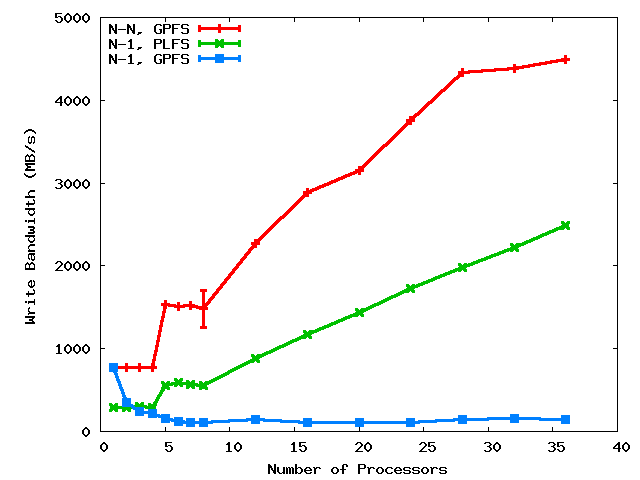
\includegraphics[width=0.4\textwidth]{data/overhead/gpfs.eps}
    \mycaption{fig-overhead}{Overhead.}{
        Ideally, N-1
        patterns written through \plfs\ would be able to 
        achieve the bandwidth available to an N-N pattern
        written directly to the \upfs.  However, 
        this graph shows that various overheads make this
        difficult.  Even though
        there is overhead, the important
        point is that \plfs\ still allows an N-1 pattern to
        be written much more quickly than if it was written
        directly to the \upfs. 
        \vspace{.5cm}
    }
\end{SCfigure}


As was seen in
Figures~\ref{eval:panfs},~\ref{eval:gpfs},~and~\ref{eval:lustre}, N-1 patterns
written through \plfs\ only match the bandwidth achieved by N-N patterns
written directly to the \upfs\ once the storage system bandwidth is saturated.
For small number of processes, \plfs\ cannot match the performance of N-N
(nonetheless, it does still improve bandwidth over a direct N-1 pattern). This
overhead is measured in Figure~\ref{fig-overhead} which shows results as
measured on LANL's GPFS system. In order to measure the both overhead incurred
by FUSE as well as any additional overhead incurred by \plfs, we developed a
second FUSE file system, \Term{\noopfs}.  \noopfs\ does no extra work, merely
redirecting all IO to the \upfs (\ie\ GPFS). For those readers familar with
FUSE, please note that \noopfs\ caches the file descriptor created in the
\syscall{open} into the opaque FUSE file handle pointer, uses it for subsequent
\syscall{writes} and \syscall{reads}, and closes it in the \syscall{flush}.

Figure~\ref{fig-overhead} is almost the same as Figure~\ref{eval:gpfs} which
compares the bandwidths measured for N-N directly to GPFS, N-1 directly to
GPFS, and N-1 indirectly to GPFS written through \plfs. The difference here is
that several new measurements have been added. The first is for N-N written
indirectly to GPFS through \noopfs. This line is significantly lower than the
line for N-N written directly to GPFS; the delta between these lines is the
overhead incurred due to FUSE, which is approximately 20\%. The next
measurement added is running an N-N workload through \plfs; this shows the
additional overhead incurred by \plfs, approximately 10\%. 
The delta beween that line and the existing N-1 through \plfs\
measurements show additional overhead which we believe is due to serializations
within FUSE due to multiple processes accessing the same path within FUSE's
file table (approximately another 10\% loss). For completeness, we also
measured the bandwidth achieved by an N-1 workload written through \noopfs;
therefore, the bottom two lines on the graph provide another view of the
overhead lost to FUSE.

Although this graph shows a total overhead cost of about 40 to 50\%, this loss
of potential bandwidth is not unduly concerning. As was seen in
Figure~\ref{eval:panfs}, the loss of potential bandwidth due to this overhead
disappears for reasonable HPC processor counts. Even with a limited per-node
bandwidth, a relatively small number of nodes writing through \plfs\ is able to
saturate the storage bandwidth. 


\subsection{Beyond Writing}
Although \plfs\ is designed primarily for {\em writing} checkpoints,
checkpoint files are still occassionally read.
We must therefore weigh improvements in 
write bandwidth against possible degradations in other operations. 

\subsubsection{Read Bandwidth}
\begin{figure*}[tb]
    \centering
        \readgraph{Uniform Restart}{nn}{data/reads/nn.eps}
        \readgraph{Non-uniform Restart}{nm}{data/reads/nm.eps}
        \readgraph{Archive Copy}{n1}{data/reads/archive.eps}
    \\
    \mycaption{fig-reading}{Read Bandwidth.}{
These three graphs show the results of our read measurements on the
\rrz. We created a set 20~\GB\ N-1 checkpoint files through
\plfs\ and another directly on PanFS.  Each file was produced by a different
number of writers; all of the \syscall{writes} were 47001 bytes in size.  For
each graph, the \yaxis\ shows the read bandwidth as a function of the number of
writers who created the file.  The graph on the left shows the read bandwidth
when the number of readers is the same as the number of writers, as is the case
in a typical uniform restart; in this case, the size of the reads is the same
as the size of the original writes.  The graph in the middle emulates a
non-uniform restart in which the application resumes on one fewer compute
nodes; in this case, the size of the \syscall{reads} is slightly larger than
the size of the original \syscall{writes}.  Finally, the graph on the right
shows the read bandwidth when there only four readers; we used LANL's archive
copy utility and modelled the common scenario of copying checkpoint data to an
archive system using a relatively small number of readers.  To enable
comparison across graphs, the axis ranges are consistent.
} 

\end{figure*}



To ensure \plfs\ does not improve write bandwidth at the expense of read
bandwidth, we ran a set of read experiments on \rrz\ which are shown in
Figure~\ref{fig-reading}. We first created two sets of 20~\GB\ files, each
written by a different number of writers; all writes were 47001 bytes (in other
words, increasing numbers of writers issued decreasing numbers of writes). One
set was created directly on PanFS; the other indirectly through \plfs. In all
cases, reads were performed on different nodes than those where the
corresponding data was written and caches were always flushed between
successive reads.

We measured the time to read these files using three different read
scenarios. One emulates a \Term{uniform restart} in which the number of
processes resuming the application is the same as the number that wrote the
last checkpoint. In this case, each rank within the parallel job reads the
same data in the same order as the previous writer of that same rank. In
contrast, a \Term{non-uniform restart} is one in which the number of
readers is different from the number of writers and the read offsets are
therefore not aligned with the previous writes. In this case, we emulate the
scenario where an application resumes after a failure by simply running on the
newly reduced number of nodes. The number of reads is not affected by the size
of the job for typical N-1 checkpoints. Each read is extracting a region for a
particular variable within the simulation. The size of this region depends on
the number of processes within the job. Each gets $1/Nth$ of the region.
Specifically, for a non-uniform restart in which the number of processes, $N$,
has been reduced by $M$, the size of each read will be $N/(N-M)$ times the size
of the original writes. The third read scenario we emulated is a typical
scenario in which a relatively, small fixed number of processes reads a
checkpoint in order to save it onto an archive system. For these measurements,
we used LANL's archive copy utility with fours readers each running on their
own node; each reader read just one contiguous 5~\GB\ region by issuing 
sequential 1~\MB\ reads. 

\if 0
% tempting to say this but we said at the beginning that we wouldn't really
% talk about segmented anymore
The archive copy uses an N-1 segmented pattern to
read a checkpoint that was written with N-1 strided.
\fi

The results of these experiments can be seen in Figure~\ref{fig-reading}. In
order to allow comparison across the three experiments, the ranges of the axes
have been made consistent. The \yaxis\ shows read bandwidth as a function of
the number of writers who created the checkpoint. We can easily see from these
graphs that the highest bandwidth is achieved using \plfs\ in the uniform
restart scenario. This is not surprising: each reader moves sequentially
through just one, nonshared file, a pattern easily improved through prefetching
performed by the \upfs. The bandwidth decreases here due to the decreasing
amount of data read as the number of readers increases. With less data read by
each, the open times begin to dominate, and there is less potential for
prefetching. The very low bandwith observed when the checkpoint is stored
directly on PanFS is also not surprising due to its layout of data within RAID
groups. Each contiguous \GB\ is spread only across a single RAID group (in this
case consisting of just eight storage devices from a pool of around one
hundred). The nature of the N-1 pattern and the size of the reads means that
all readers will almost always be reading within just a single RAID group. In
addition to limiting the bandwidth to only a few storage devices, it also
reduces the bandwidth from each of them due to overloading them with
non-sequential requests.

The results for the non-uniform restart can be similarly explained. The PanFS
results and explanation are essentially the same. The results for \plfs\ are
also very similar; better than PanFS due to spreading the reads across all
storage devices and not quite as good as the \plfs\ results for the uniform
restart. The difference between the uniform and non-uniform results for \plfs\
is only seen for small numbers of readers in the area where \plfs\ was helped
by prefetch in the uniform experiment. Since the readers are reading different
offsets than were written in the non-uniform restart, they will read multiple
data files instead of just reading a single one. The \upfs, unsurprising,
does not identify this admittedly strange pattern and therefore there is no
prefetch benefit. Only when there is no longer any prefetch benefit, 
do these results converge.

Although we are pleased to see that \plfs\ also does relatively well for the
archive copy experiment, we do not yet fully understand all of these results.
We can think of no reason why the bandwidths should be this low and we assumed
that PanFS would easily outperform \plfs\ due to having contiguous data within
its RAID groups instead of having data spread across multiple data files
within a \plfs\ container.  However, we are not surprised to see the read
bandwidths drop as the number of writers increases.  Increasing numbers of
writers results in a data layout with fewer large contiguous regions of data
for both \plfs\ and PanFS; therefore, the read bandwidth will suffer
accordingly.

%this behavior has been
%independently observed thrice that we know of: once by us, and twice by two
%groups of students at CMU. 

\subsubsection{Metadata Queries}

As we discussed in Section~\ref{arch-meta}, there are currently two techniques
used to discover the metadata for a \plfs\ file. For a file being currently
written, metadata is discovered by \syscall{stat'ing} individual data files.
When a file is closed, metadata information is cached as file names within a
specific subdirectory inside the container. Thereafter, metadata information
can be discovered merely by issuing a \syscall{readdir}. Obviously, the first
technique is much slower; if our primary interest was in optimizing metadata
query rates, than we could cache this metadata following every write. However,
since \plfs\ is designed for checkpoint writing, we do not consider this
technique.

Figure~\ref{fig-metadata} compares these two times against the time it takes to
query a closed file written directly to the \upfs, PanFS. We have not yet
measured the time to query an open file on PanFS. For this experiment,
conducted on LANL's \rrz, we created two sets of 20~\GB\ files each written by
a different number of writers all issuing 47001 byte-sized writes. One set was
created directly on PanFS; the other indirectly through \plfs.  As the graph
shows, the \syscall{stat} times for closed files on \plfs\ and PanFS are
approximately the same.  However, as expected, the time to query a \plfs\ file
open for writing is greater than to query a closed file.

%plateaus for \plfs may be due to \Term{statahead} in the PanFS client.
%We suspect this is due to the small number of writers available on
%the \rrz; we hope to rerun this experiment on Roadrunner itself. 

\begin{figure}
    \centering
    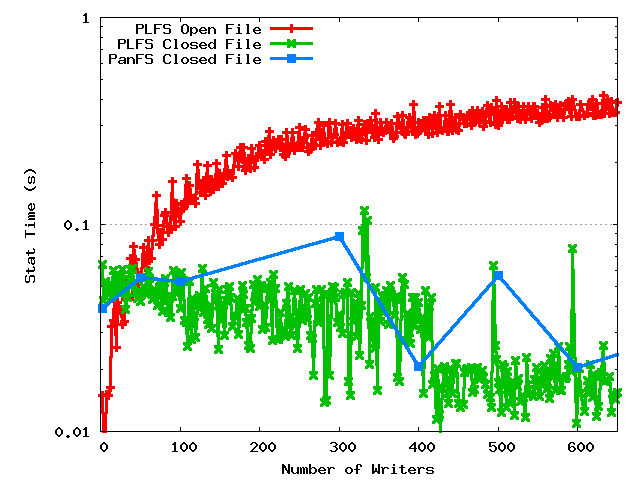
\includegraphics[width=0.4\textwidth]{data/stat/stat.eps}
    \mycaption{fig-metadata}{Metadata Queries.}{
        This graph compares the time to \syscall{stat} a 20~\GB\ file
        on \plfs\ with the time to \syscall{stat} a comparable
        file on PanFS.    
        The \yaxis, which is in logscale,
        shows the \syscall{stat} time 
        as a function of the number of writers who created that
        file.  We compare the PanFS \syscall{stat} rate to the
        \plfs\ rate for files opened for writing, and to the 
        \plfs\ rate for closed files.
        \vspace{1cm}
    }
\end{figure}


% What's up with the weird data for the stat time on an open PLFS file?
% I thought maybe it had to do with the number of subdirectories so I
% reran it with 999 subdirectories and it didn't change. Not sure now.

\section{Related Work}
\label{related}

% Remzi says refer to Erez Zadok's work on stackable file systems
% also says to refer to Thain's interposition work.  But we already did.

%Sudharshan Vazhkudai has several papers on checkpointing, typically using
%memory or scavenged local disk as a buffer.  Descriptions available at his
%webpage: \url{http://www.csm.ornl.gov/~vazhkuda/}.

%Frank Shorter's Master Thesis at Clemson is a big discussion about parallel
%benchmarks: \url{ftp://ftp.parl.clemson.edu/pub/techreports/2003/PARL-2003-001.ps}.

Translating random access checkpoint writes into a sequential pattern is an
idea which extends naturally from work on log-structured file
systems~\cite{lfs} such as NetApp's WAFL~\cite{WAFL} and Panasas's Object
Storage~\cite{welch08scalableperformance}. While these ideas reorganize disk
layout for sequential writing, they do not decouple concurrency caused by
multiple processes writing to a single file.  Another approach to
log-structuring N-1 patterns addressed only physical layout and also did not
decouple concurrency~\cite{pvfs-log}.  We believe our contribution of
rearranging N-1 checkpoints into N-N is a major advance. 

Checkpoint-restart is an old and well studied fault tolerance strategy. A broad
evaluation of rollback-recovery protocols and checkpointing and a discussion of
their future at the petascale can be found in \cite{survey1, survey2}.  

Berkeley Lab Checkpoint/Restart~\cite{blcr} and Condor
Checkpointing~\cite{condor-ckpt} both allow unmodified applications to
checkpoint the state of a single node.  They leverage the operating system's
ability to swap a process to save the totality of the swap image persistently.
The great strength of this approach is that it can be used by applications that
have no internal checkpoint mechanism.  A disadvantage is that these
checkpoints are larger then when an application specifies only the exact data
that it needs saved.
Conversely, incremental checkpointing and memory
exclusion~\cite{pcl:99:me,pxn:95:scd} reduce the size of checkpoint data by
only saving data that has changed since the previous checkpoint.  Buffering
with copy-on-write~\cite{li-298215} can also reduce checkpoint latency.

%allows user applications to checkpoint their state, including system
%resources, without the application programmer having to explicitly code the
%process. In this regard, it has a similar philosophy to \plfs\ of making
%checkpointing easier for the application developer, but our focus is on
%enabling better checkpointing performance for existing applications rather than
%writing an entire checkpointing system.  

%\scribble{Couldn't find the incremental checkpointing reference}


\newcommand{\C}[1]{\centering{#1}}
%\newcommand{\C}[1]{\begin{center}#1\end{center}}
\hyphenation{Immediately}
\begin{table*}
\begin{center}
\begin{tabular}{|r|p{19mm}|p{20mm}|p{23mm}|p{15mm}|p{19mm}| p{19mm}|}
\hline 
{\em } & 
\C{{\em Interposition Technique Used}} & 
\C{{\em No Extra Resources Used During}} & 
\C{{\em No Extra Resources Used After}} & 
\C{{\em Maintains Logical Format}} & 
\C{{\em Works with Unmodified Applications}} & 
\C{{\em Data Immediately Available}} 
\tabularnewline \hline
ADIOS & \C{Library} & \C{Yes} & \C{Yes} & \C{Yes} &  \C{No} & \C{Yes}
\tabularnewline \hline
{\tt stdchk} & \C{FUSE} & \C{No (LD, M)} & \C{No (LD, N, M)} & \C{Yes} & \C{Yes} & \C{Yes}
\tabularnewline \hline
%Neighbor &  \C{FUSE} &\C{No (M)} & \C{No (M, N)} & \C{Yes} & \C{Yes} & \C{Yes} 
%\tabularnewline \hline
Diskless &  \C{Library} &\C{No (M)} & \C{No (M)} & \C{No} & \C{No} & \C{Yes} 
\tabularnewline \hline
Sp Writ &  \C{Library} &\C{Yes} & \C{Yes} & \C{Yes} & \C{No} & \C{No} 
\tabularnewline \hline
ZEST &  \C{FUSE} &\C{No (RD)} & \C{No (RD)} & \C{No} & \C{No} & \C{No} 
\tabularnewline \hline
PLFS & \C{FUSE} & \C{Yes} & \C{Yes} & \C{Yes} & \C{Yes} & \C{Yes} 
\tabularnewline \hline
\end{tabular}
\mycaption{tab-feature}{Techniques for improving N-1 Checkpointing}{
This table presents a comparison of the various techniques for reducing
N-1 checkpoint times.  For exposition, we have used various
shorthands: 
%Neighbor for Neighbor's Memory,
Diskless for Diskless 
Checkpointing, Sp Writ for Lustre Split Writing, LD for local disk on the compute nodes, RD for remote disk 
on the storage system, M for memory, and N for network.  
}
\end{center}
\end{table*}

\if 0
other possible columns:

            Speed
    ADIOS: Disk                                                                 
    stdck: Disk                                                                 
    Neighbor: Network                                                           
    Diskless: Network                                                           
    ZEST: Spindle                                                               
    PLFS: N-N  

lines of code, user or kernel mode, interposition technique, maintainability,
portability

also if we add more columns we'll have to rotate it so columns become rows and
rows become columns.

\fi


%A variant of N-N checkpoint uses the disks or memory of computer nodes to
%record a checkpoint writing it to storage as a background process during the
%next compute period. 

{\tt stdchk}~\cite{stdchk} saves checkpoints into a cloud of free disk space
scavenged from a cluster of workstations.  A similar
approach~\cite{aggregate-memory} reserves compute node memory to temporarily
buffer checkpoints and then asynchronously saves them to persistent storage.
Diskless checkpointing~\cite{diskless} also  
saves checkpoints into compute node memory, but does not subsequently transfer
them to persistent storage.  Rather it achieves fault protection by using erasure 
coding on the distributed checkpoint image. 
Although these techniques work well for many applications, large HPC parallel
applications jealously utilize all memory and demand a high degree of
determinism in order to avoid jitter~\cite{DusseauPhd98} and are therefore seen
to be poorly served by techniques reducing available memory or techniques which
require background processes running during computation.

The Adaptable IO System (ADIOS)~\cite{adios} developed by the Georgia Institute
of Technology and Oak Ridge National Laboratory provides a high-level IO API
that can be used in place of HDF5 to do much more aggressive write-behind and
log-like reordering of data location within the checkpoint. While this technique
requires application modification, it enables interoperability with other
middleware libraries.  Similarly, Lustre Split Writing~\cite{lsw}, uses a 
library approach and leverages Lustre's file joining mechanism to decouple
concurrent access at runtime as does \plfs.  However, Lustre Split Writing is
wed to the Lustre file system, requires application modification, and prevents
the data from being immediately available following a checkpoint.

ZEST~\cite{zest}, developed at Pittsburgh Supercomputing Center, is a file
system infrastructure that is perhaps the most similar in philosophy to \plfs,
particularly in its borrowing of concepts from log-structured file systems.
Rather than each client process pushing their writes sequentially to storage,
in ZEST manager threads running on behalf of each disk pull data from a series
of distributed queues, in a technique borrowed from
River~\cite{Arpaci-Dusseau03-TOCS}.  The key aspect of ZEST is that no
individual write request is ever assigned to a specific disk; disks pull from
these queues whenever they are not busy, resulting in high spindle utilization
even in a system where some devices are performing more slowly than others.
Unlike \plfs, however, data is not immediately available to be read, requiring
a subsequent phase to first rewrite the file before it can be accessed.  Since
this phase happens in the relatively long time between checkpoints and since it
happens on the server nodes and not on the compute nodes, this subsequent
rewrite phase is not typically problematic for a dedicated checkpoint file
system.

\section{Current Status and Future Work}
\label{future}

\scribble{I removed the 'cute' part of this. Sorry, john}
We initially developed \plfs\ in order to test our hypothesis that an
interposition layer could rearrange checkpoint patterns such that the
convenience of N-1 patterns could be preserved while achieving the bandwidth of
N-N.  However, after achieving such large improvements with real LANL
applications, we were compelled to harden it 
into a production file system. Consisting of about three thousand lines of
code, \plfs\ is currently an optional mount point on Roadrunner where several
applications have begun using it to improve their N-1 checkpoint performance. 
\plfs\ is publically available at
http://sourceforge.net/projects/plfs.

%Since \plfs\ consists of only three thousand
%source lines of code and is easily ported to all Linux architectures, we
%decided~\footnotemark that the costs of maintaining it are easily outweighed by
%the benefits.
%\footnotetext{were persuaded by management}

Although \plfs\ works transparently with unmodified applications, in practice
some applications may need to make minor changes.  Many users find it most
convenient to stage their input data sets and their executable code in the same
directory where they write their checkpoint files.  Since \plfs\ is
specifically a checkpoint file system and is not a general purpose file system,
this usage pattern may suffer a performance hit.  These users should instead
stage their input data sets and their executable code in a general purpose file
system and merely direct their N-1 checkpoint files to \plfs.

Also, applications that open \plfs\ files in read-write mode will find that
reading from these files can be very slow.  As we discussed in
Section~\ref{arch-read}, reads in \plfs\ are handled by reading and aggregating
the index files.  When files are opened in write-read mode, this process must
be repeated for every \syscall{read} since intervening \syscall{writes} may
have occurred.  Although the vast majority of HPC applications are able to read
in read-only mode, we do plan to investigate removing this limitation in the
future for those few applications who must occasionally read while writing.
One possibility is to introduce metadata servers which can synchronously
maintain an aggregated index in memory. 

Originally intended merely to address N-1 challenges, \plfs\, as currently
designed, also has the potential to address N-N challenges.  One way that
\plfs\ can reduce N-N checkpointing times is by reducing disk seeks through its
use of log-structured writing.  However, we have yet to measure the
frequency of non-sequential IO within N-N checkpoints.

\scribble{Added gigaplus reference to the end. --Milo}
Another challenge of an N-N pattern is the
overwhelming metadata pressure resulting from the simultaneous creation of tens
of thousands of files within a single directory.  Currently HPC parallel file
systems do distribute metadata across multiple metadata servers; however they do so
at the granularity of a \Term{volume} or a directory (\ie\ all files within a
directory share a single metadata server).  \plfs\ can easily refine this
granularity by distributing container subdirectories 
across multiple metadata servers.  At the moment, \plfs\ only creates container
structures for regular files; directories are simply created directly on the
\upfs.  By extending \plfs\ to create a similar container structure for
directories, we believe that \plfs\ can effectively address this N-N challenge
as well, in a manner similar to~\cite{gigaplus}.

\section{Conclusion}
\label{conclude}

Large systems experience failures.  To protect themselves against these
failures, parallel applications running on these systems save their progress by
checkpointing.  Unfortunately for many of these applications, their preferred
checkpointing patterns are extremely challenging for the \upfs\ and impose
severe bandwidth limitations.  In this paper, we have developed \plfs\ to
demonstrate how a simple interposition layer can transparently rearrange these
challenging patterns and improve checkpoint bandwidth by several orders of
magnitude.

The parallel file system attached to Roadrunner is the largest LANL has ever
had; testing it has revealed that the challenges of N-1 patterns are severely
exacerbated at this scale.  Given current bandwidths, we know of no current N-1
application at LANL that can effectively checkpoint across the full width of
Roadrunner.  \plfs\ allows them to do so. 

\clearpage

%\clearpage
\singlespace
% tiny is smaller than scriptsize
{\scriptsize
    \bibliographystyle{abbrv}
    \bibliography{defs,all}
}

\end{document}
